\documentclass[xcolor=table]{beamer}

\usepackage{booktabs}
\usepackage{hyperref}
\usepackage[table]{xcolor}
\usepackage{tikz}
\usepackage{graphics}
\usetikzlibrary{calc}

\setbeamertemplate{navigation symbols}{}%remove navigation symbols

\title{Incomplete information}
\subtitle{Game Theory}
\author{Vincent Knight}
\date{}

\begin{document}

\frame{\titlepage}

\frame{
\tikzstyle{level 1}=[level distance=2.5cm, sibling distance=3.5cm]
\tikzstyle{level 2}=[level distance=2.5cm, sibling distance=2cm]
\tikzstyle{level 3}=[level distance=2.5cm, sibling distance=1cm]
\tikzstyle{player} = [text width=4em, draw, text centered, rectangle, fill=blue!20, inner sep=1pt]
\tikzstyle{nature} = [minimum width=3pt,circle,  draw, fill=red!20, inner sep=1pt]
\tikzstyle{end} = [circle, minimum width=3pt, fill, inner sep=0pt, right]
\begin{center}
\begin{tikzpicture}[grow=right, sloped]
    \node[nature]{Card}
        child { node[player] {P1}
            child{ node[end] {} node[right] {$(-3,1)$}  edge from parent node[below] {Red}}
            child{ node[player] (A) {P2}
                child{ node[end] {} node[right] {$(4,-2)$} edge from parent node[below] {Blue}}
                child{ node[end] {} node[right] {$(-4,1)$} edge from parent node[below] {Red}}
            edge from parent node[below] {Blue}}
        edge from parent node[above] {.25} node[below] {Tails}}
        child { node[player] {P1}
            child{ node[player] (B) {P2}
                child{ node[end] {} node[right] {$(1,-3)$} edge from parent node[below] {Blue}}
                child{ node[end] {} node[right] {$(2,-3)$} edge from parent node[below] {Red}}
            edge from parent node[below] {Blue}}
            child{ node[end] {} node[right] {$(1,-1)$}  edge from parent node[below] {Red}}
        edge from parent node[above] {.75} node[below] {Heads}}
        ;
        \draw [dashed] (A) -- (B);
\end{tikzpicture}
\end{center}
}

\frame{
\tikzstyle{level 1}=[level distance=2.5cm, sibling distance=3.5cm]
\tikzstyle{level 2}=[level distance=2.5cm, sibling distance=2cm]
\tikzstyle{level 3}=[level distance=2.5cm, sibling distance=1cm]
\tikzstyle{player} = [text width=4em, draw, text centered, rectangle, fill=blue!20, inner sep=1pt]
\tikzstyle{nature} = [minimum width=3pt,circle,  draw, fill=red!20, inner sep=1pt]
\tikzstyle{end} = [circle, minimum width=3pt, fill, inner sep=0pt, right]

\begin{center}
\begin{tikzpicture}[grow=right, sloped, scale=.6, every node/.style={scale=0.6}]
    \node[nature]{Card}
        child { node[player] {P1}
            child{ node[end] {} node[right] {$(-3,1)$}  edge from parent node[below] {Red}}
            child{ node[player] (A) {P2}
                child{ node[end] {} node[right] {$(4,-2)$} edge from parent node[below] {Blue}}
                child{ node[end] {} node[right] {$(-4,1)$} edge from parent node[below] {Red}}
            edge from parent node[below] {Blue}}
        edge from parent node[above] {.25} node[below] {Tails}}
        child { node[player] {P1}
            child{ node[player] (B) {P2}
                child{ node[end] {} node[right] {$(1,-3)$} edge from parent node[below] {Blue}}
                child{ node[end] {} node[right] {$(2,-3)$} edge from parent node[below] {Red}}
            edge from parent node[below] {Blue}}
            child{ node[end] {} node[right] {$(1,-1)$}  edge from parent node[below] {Red}}
        edge from parent node[above] {.75} node[below] {Heads}}
        ;
        \draw [dashed] (A) -- (B);
\end{tikzpicture}
\end{center}
$$S_1=\{\text{RedRed},\text{RedBlue},\text{BlueRed},\text{BlueBlue}\}\text{ and }S_2=\{\text{Red},\text{Blue}\}$$
\pause
$$\begin{pmatrix}
(0,-.5)&(0,-.5)\\
(.25,-.5)&(1.75,-1.25)\\
(.75,-2)&(0,-2)\\
(.5,-2)&(1.75,-2.75)\\
\end{pmatrix}$$
}

\frame{
\begin{center}
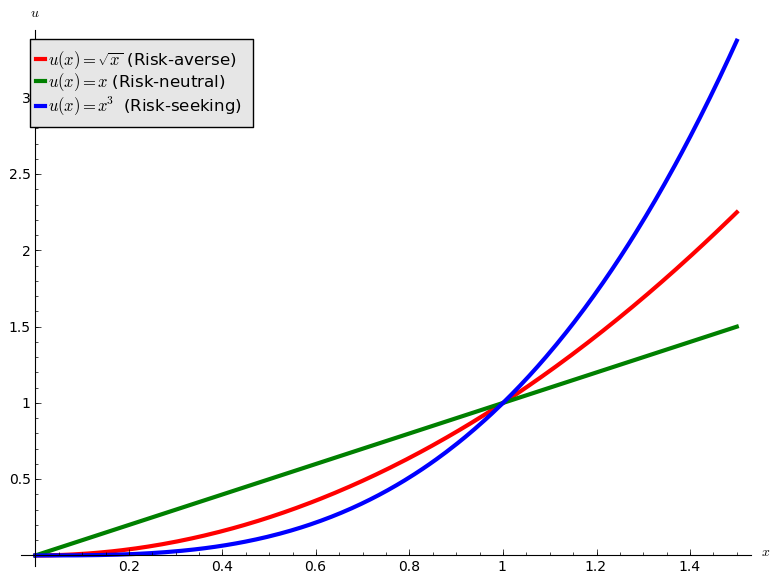
\includegraphics[width=.8\textwidth]{../Course_Notes/plots/L13-plot01.png}
\end{center}
}

\end{document}
